\chapter{Reference abstract software architecture}
\label{software-arch}

\section{Overall architecture}

\begin{figure}[htbp]
  \centering
  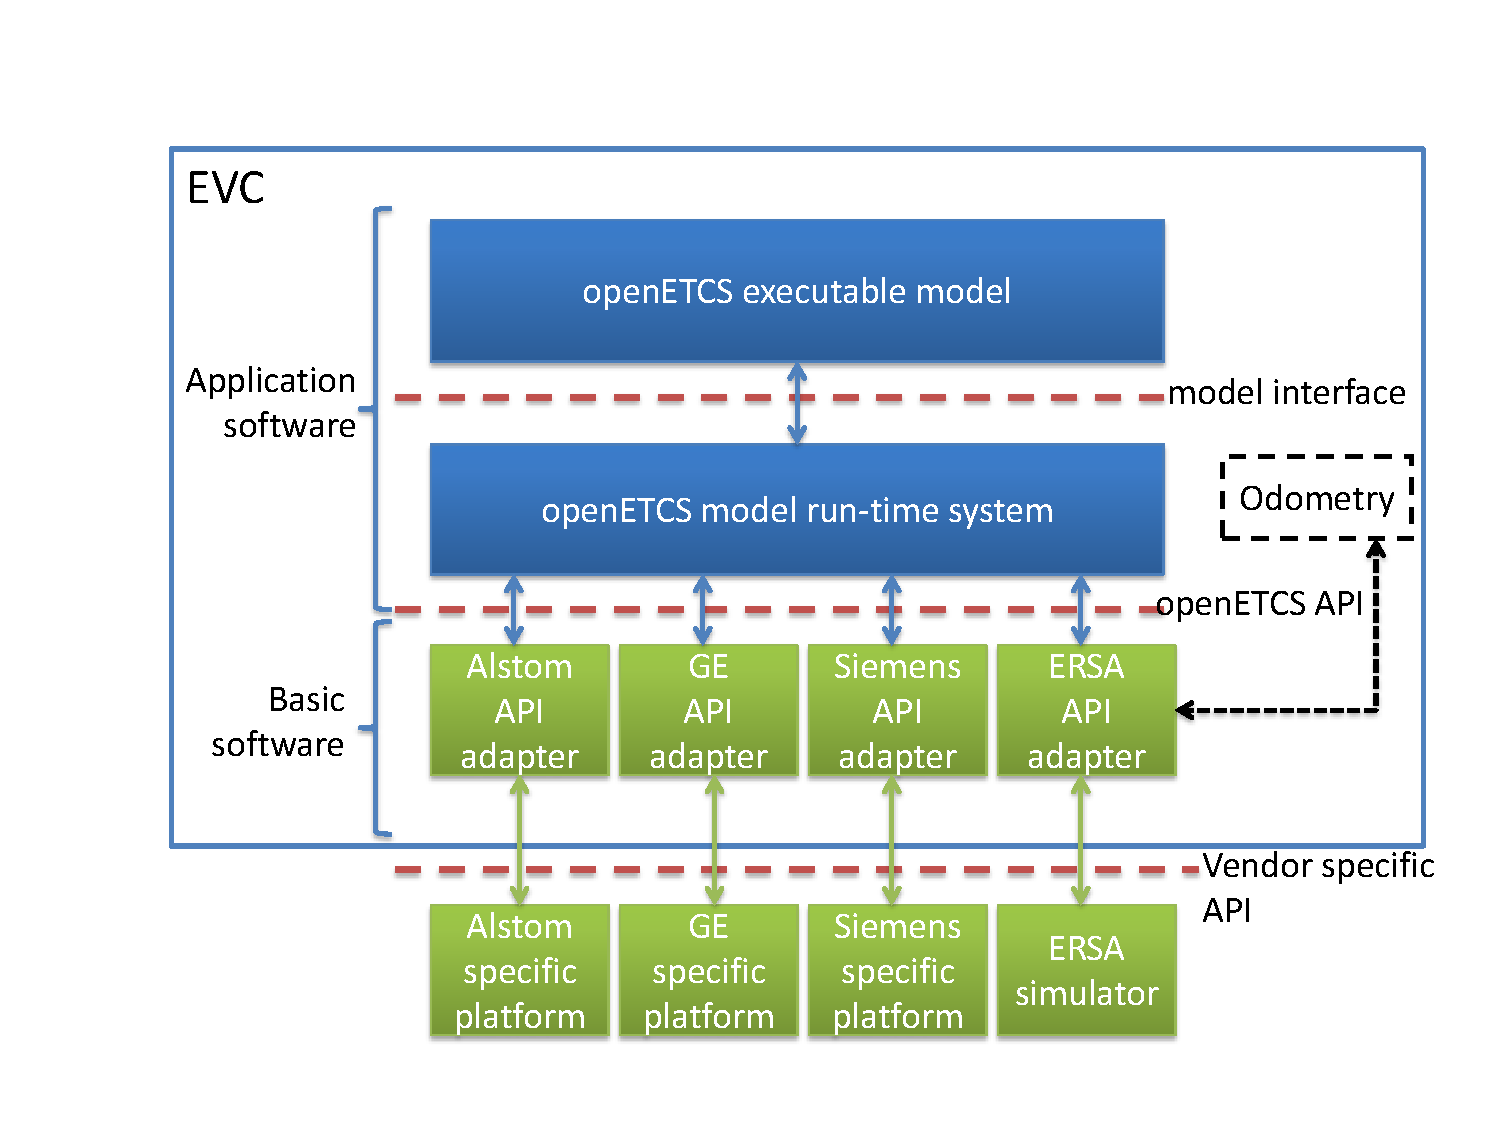
\includegraphics[width=\linewidth]{software-architecture.pdf}
  \caption{Reference abstract software architecture}
  \label{fig:software-arch}
\end{figure}

The \define{reference abstract software architecture} is shown in figure
\ref{fig:software-arch}. This architecture is made of following
elements:
\begin{itemize}
\item \define{openETCS executable model} produced by the
  \cite{scade-model}. It shall contain the program implementing core
  ETCS functions;
\item \define{openETCS model run-time system} shall help the execution
  of the openETCS executable model by providing additional functions
  like encode/decode messages, proper execution of the model through
  appropriate scheduling, re-order or prioritize messages, etc. This
  block shall be described in another openETCS document. \FIXME{ref?}
\item \define{Vendor specific API adapter} shall make the link between
  the Vendor specific platform and the openETCS model run-time system.
  It can buffer message parts, encode/decode messages, route messages
  to other EVC components, etc.
\item All above three elements shall be included in the EVC;
\item \define{Vendor specific platform} shall be all other elements of
  the system, bus and other units, as shown in figure
  \ref{fig:hardware-arch}.
\end{itemize}

We have thus three interfaces:
\begin{itemize}
\item \define{model interface} is the interface between openETCS
  executable model and openETCS model run-time system. It shall be
  described in another openETCS document \FIXME{ref?};
\item \define{openETCS API} is the interface between openETCS model
  run-time system and Vendor specific API adapter. It is described in
  this document;
\item \define{Vendor specific API} is the interface between Vendor
  specific API adapter and Vendor specific platform. This interface is
  not publicly described.
\end{itemize}

The two blocks openETCS executable model and openETCS model run-time
system are making the \define{Application software} part. This
Application software might be either openETCS reference software or
vendor specific software.

The Vendor specific API adapter is making the \define{Basic software}
part.

\section{Information exchange between blocks}

At this level of description, we do not explain how the various blocks
of above architecture are calling themselves. We only assume they are
exchanging \define{messages} in an asynchronous way. A message is a set
of information corresponding to an event of a particular unit, e.g. a
balise received from the BTM. The possible kind of messages are
described in chapter \ref{information-flows}.

How the exchange of messages in implemented in actual software,
e.g. function call, storage of data in a shared buffer, ..., is
described in chapter \ref{concrete-interface}.

\section{Architectural variations}
Please note that the reference abstract hardware and software
architectures do not forbid architectural variations. For example, the
Odometry function could be put within the EVC (see ODO on figure
\ref{fig:software-arch}) instead of a separate hardware unit (as it
was shown on figure \ref{fig:hardware-arch}). Such Odometry function
would be part of the Application software. But communication between
this Odometry function within EVC and the openETCS model run-time
system shall be done through the openETCS API and shall follow its
conventions.

As another example, part of Vendor specific platform could be on EVC
and thus the Vendor specific API would be within the EVC.


% LocalWords:  openETCS API EVC Odometry balise BTM
